\documentclass{beamer}
\usetheme{Warsaw}

\setbeamertemplate{caption}[numbered]
\usepackage{copyrightbox}

\title{Predicting the limits of the ELT}
\subtitle{Defensio}
\author[Alarich Herzner]{Alarich Herzner\\[1ex]  {\small Supervisor: Univ.-Prof. Jo\~ao Alves, PhD \\ Co-Supervisor: Dr. Kieran Leschinski, MSc}}
\institute{University of Vienna, Faculty of Physics}
\date{\today}

\begin{document}
\begin{frame}
\titlepage
\end{frame}

\begin{frame}
\frametitle{Outline}
\tableofcontents
\end{frame}

\section{Introduction}
\subsection{Goals}

\begin{frame}
\frametitle{Goals}
\begin{block}{Primary objective}
Estimate reliability limit for future IMF studies in the galactic centre using the ELT!
\end{block}
... what?
%\vspace{0.5cm}
\end{frame}

\begin{frame}
\frametitle{ELT}
  \begin{figure}
  \copyrightbox[b]{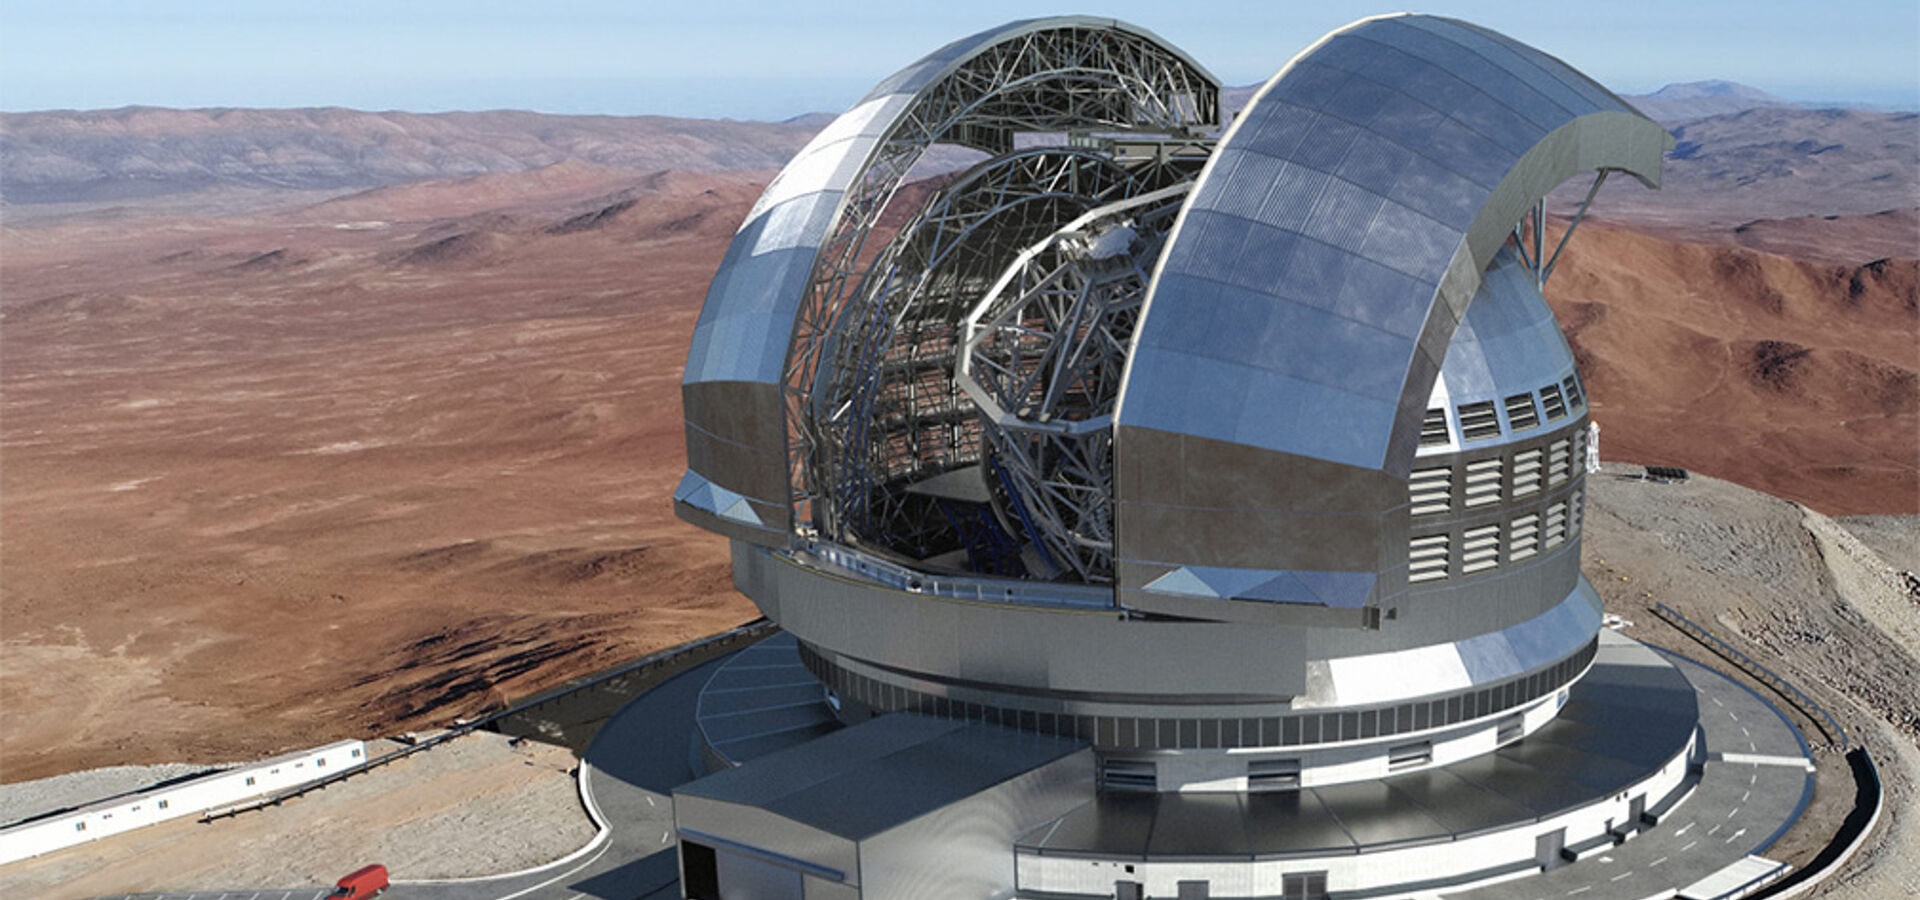
\includegraphics[width=\linewidth]{Images/ELT.jpg}}
                  {https://cdn.eso.org/images/banner1920/telescope-dome-landing.jpg}
  \end{figure}
\end{frame}

\begin{frame}
\frametitle{IMF}
  \begin{figure}
  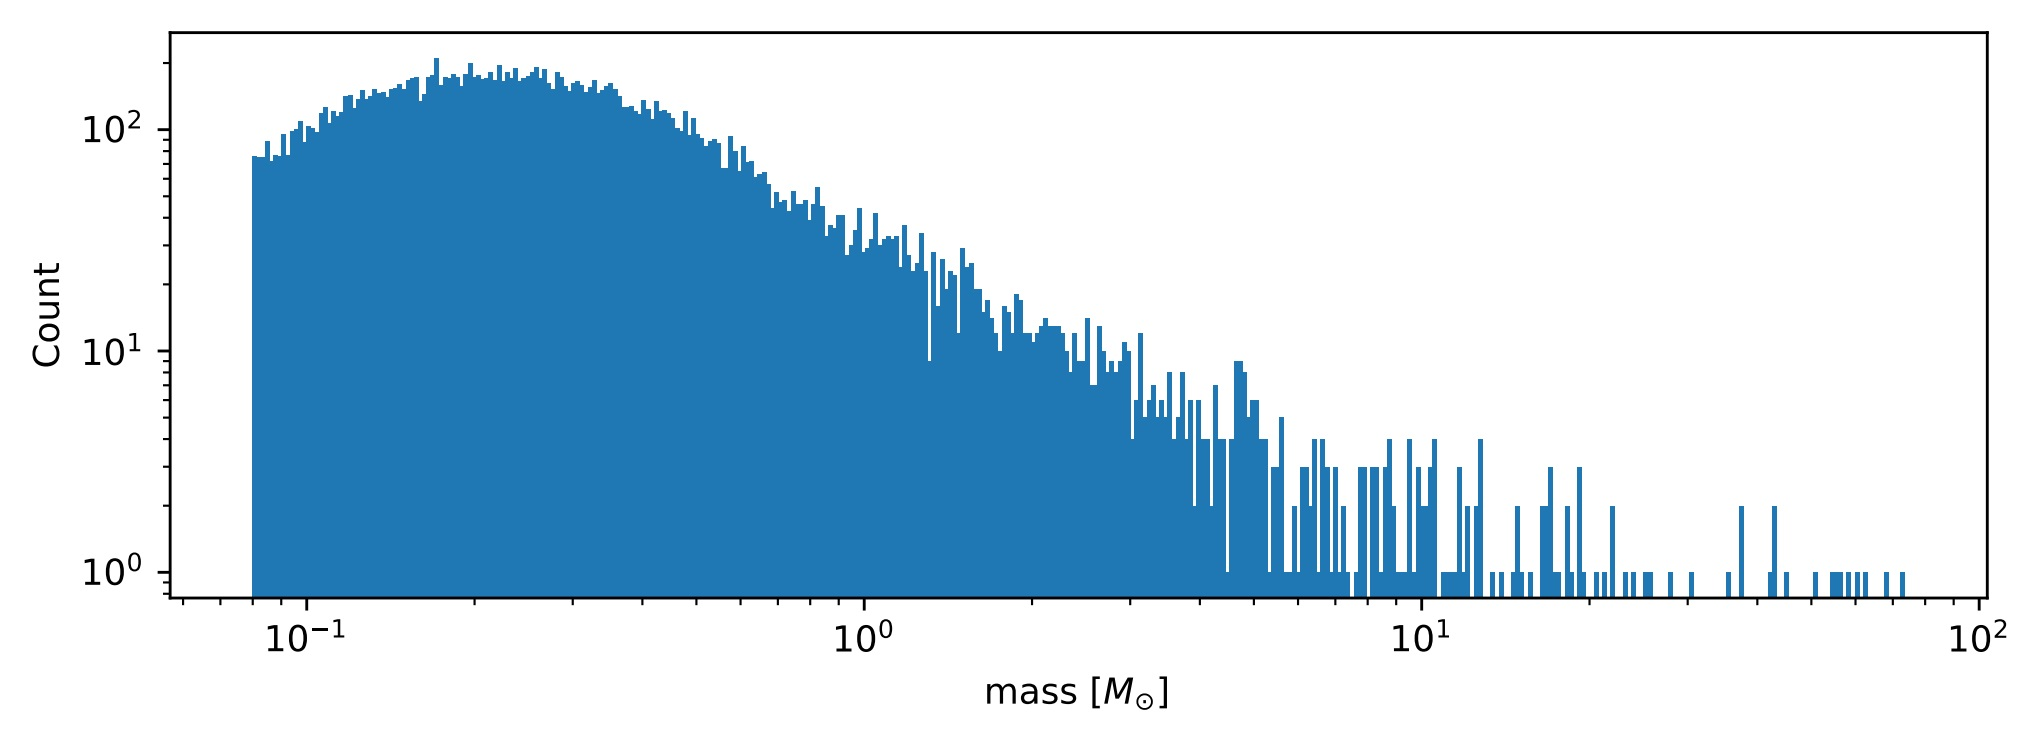
\includegraphics[width=\linewidth]{Images/IMF1.jpg}
  \end{figure}
\end{frame}

\begin{frame}
\frametitle{Reliability Limit}
  \begin{figure}
  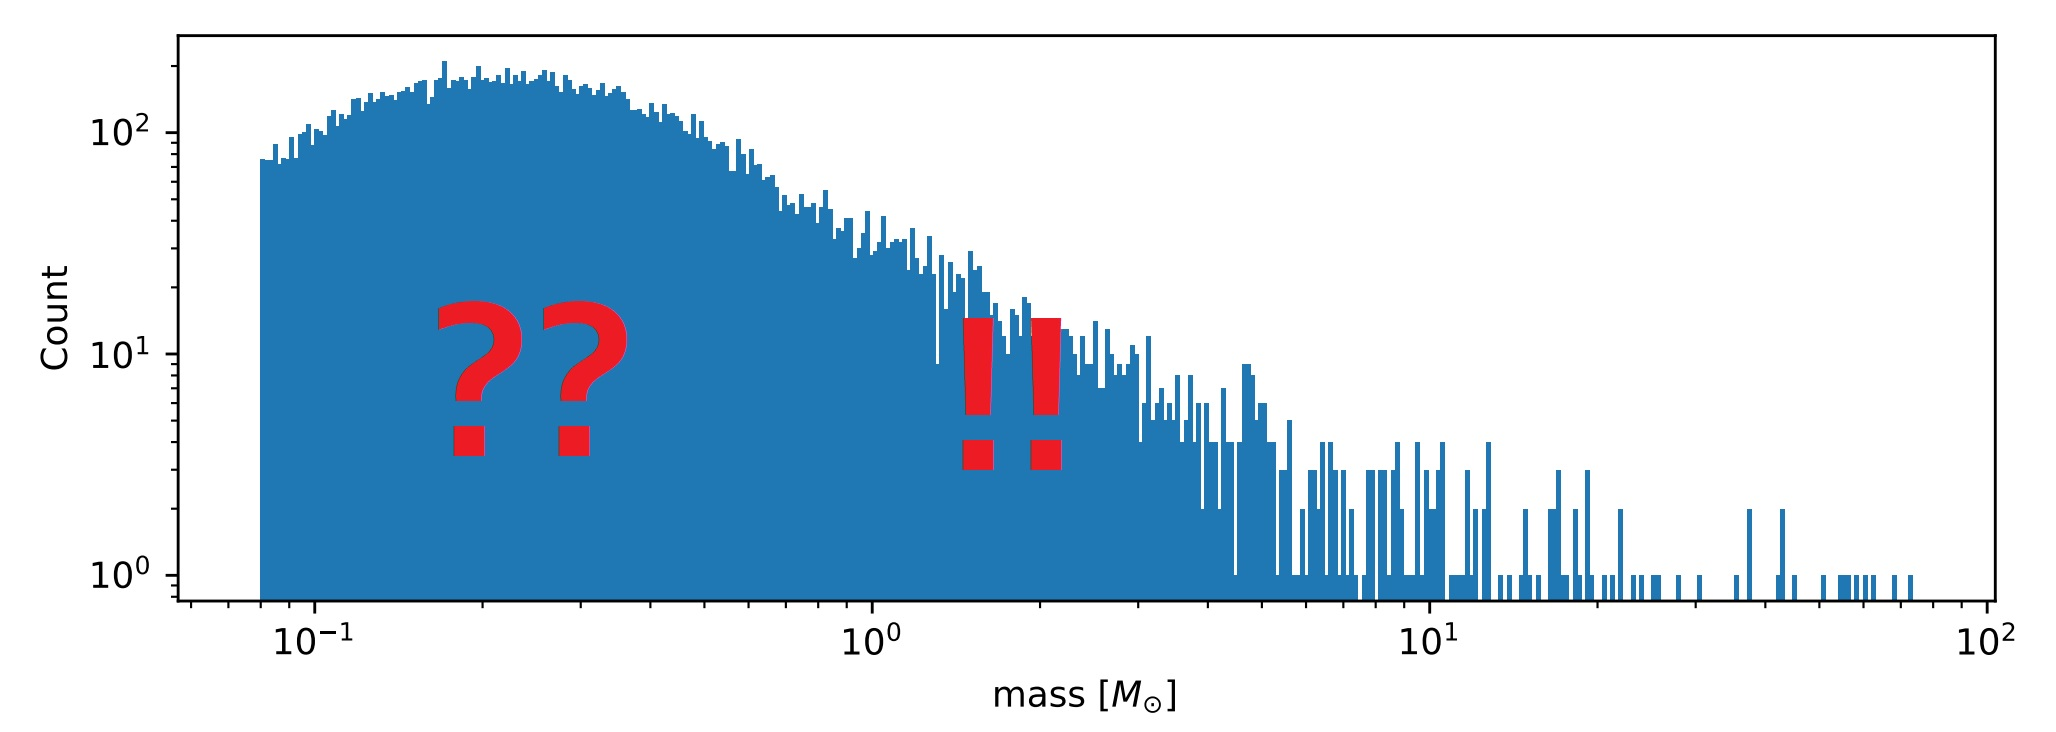
\includegraphics[width=\linewidth]{Images/IMF2.jpg}
  \end{figure}
\end{frame}


\begin{frame}
\begin{block}{Motivation}
	\begin{columns}[T]
	\column{0.48\textwidth}
	\vspace{0.5em}
	\begin{itemize}
	\item Universal IMF?
	\item estimate number of lower-mass stars
	\item understand star formation process
	\end{itemize}
	\column{0.48\textwidth}
	\vspace{0.5em}
	\begin{itemize}
	\item N-body simulation with \(N \gg 1\)
	\item Clustering of time-dependent data
	\end{itemize}
	\end{columns}
\end{block}
\end{frame}


\subsection{Action Plan}

\begin{frame}
\frametitle{Action Plan}
\begin{enumerate}[I]
\item Simulate stars
\item Observe stars
\item Analyze
\item Measure performance
\end{enumerate}
\end{frame}

\end{document}